\documentclass{article}
\usepackage[utf8]{inputenc}
\usepackage{amsmath}
\usepackage{tcolorbox}
\usepackage{indentfirst}
\usepackage{graphicx}
\usepackage{minted}
\usepackage{float}
\usepackage [english]{babel}
\usepackage [autostyle, english = american]{csquotes}
\MakeOuterQuote{"}

\title{System on a Chip Final Project Report}
\author{Jordan D Edwards}
\date{October 2023}


\begin{document}
	
	\title{Final Project
		\\ \large{ELC 4396 System on a Chip}  }
	
	\author{Jordan Edwards \\ Baylor University} %the \\ symbols starts a new line
	\date{December 11, 2023}
	\maketitle
	
	\subsection*{Introduction}
	For this assignment, I chose to integrate an ultrasonic distance sensor as an additional module. This module integrates directly into the provided bus and allows for the user to trigger a reading, get the current status of the module, and read the distance results. This project involved both System Verilog as well as C++ programming to fully implement it.
	
	\subsection*{Sensor}
	
	I used the HC-SR04 ultrasonic distance sensor for this project. The sensor has two interface pins, one for triggering a ping, and the other for receiving the results. The trigger pin expects a 5~V high-active signal for a minimum of 10~$\mu$s in order to trigger a reading. After the sensor performs its reading, the echo pin is asserted high for a number of microseconds proportional to the distance measured. This happens to be the time of flight of the acoustic wave, so the distance can be calculated by dividing by half of the speed of sound to account for the round-trip time.
	
	\subsection*{Hardware}
	
	Because the sensor uses 5V and the FPGA uses 3.3~V, some additional hardware was required in order to properly use both components. A drawing of this circuit can be found in Fig. \ref{circuit} From the echo pin of the sensor, a simple voltage divider was utilized to change the 5V signal down to 3.3~V. On the trigger pin of the sensor, the 3.3~V signal needed boosted up to 5~V. In order to accomplish this, I used an opamp in a non-inverting configuration. The gain was set to be around 5, so the 3.3~V signal had no issues pushing the output up to the 5~V rail.
	
	 \begin{figure}[H]
		\centering
		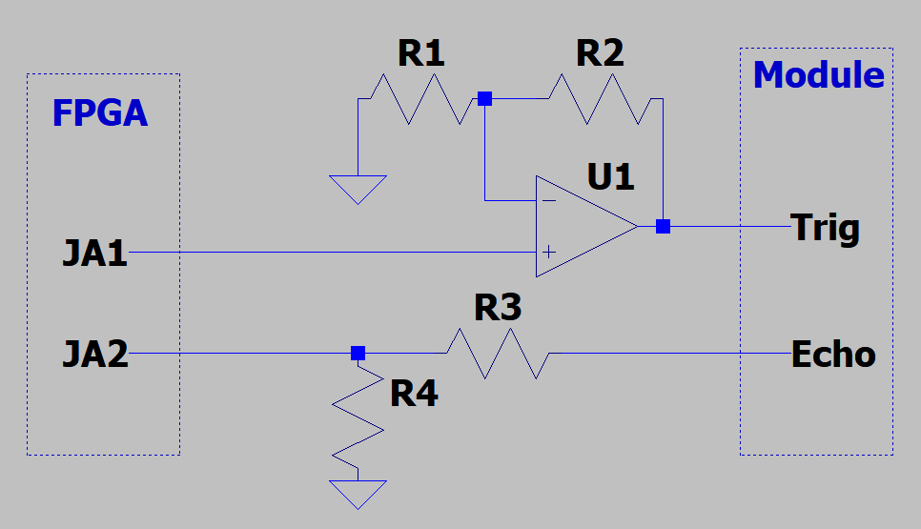
\includegraphics[width=.6\linewidth]{circuit}
		\caption{Circuit diagram for connecting the sensor to the FPGA}
		\label{fig:circuit}
	\end{figure}
	
	\subsection*{Firmware}
	
	In System Verilog, I set up a firmware core to handle talking to the sensor. This began by setting up a very simple state machine, shown in Fig. \label{states}. The goal of this state machine was to first trigger the sensor to take a reading, and then read in the result, which was presented to the module itself for access over the bus. 
	
	\begin{figure} [H]
		\centering
		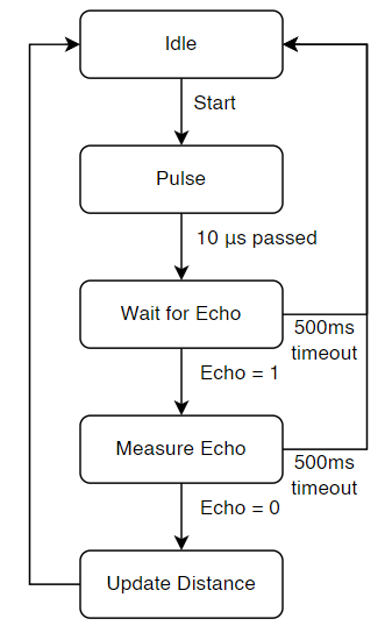
\includegraphics[width=.6\linewidth]{stateMachine}
		\caption{State machine for firmware driver}
		\label{fig:states}
	\end{figure}
	
	The bus-connected module served as an interface for connecting the direct sensor driver to the rest of the system. It interprets any write attempt as a command to update the distance, and it is capable of sending out either the most recent distance reading or a status register, which contains a ready bit as well as the number of reads the module has done so far. The interfacing code is shown in Fig. \ref{fig:interface}
	
	 \begin{figure}[H]
		\centering
		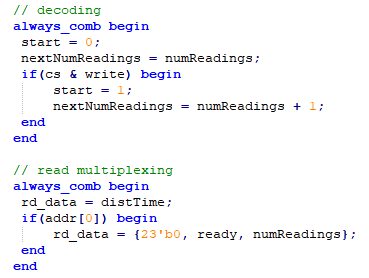
\includegraphics[width=.6\linewidth]{interface}
		\caption{System Verilog code for handling communication with the system}
		\label{fig:interface}
	\end{figure}
	
	\subsection*{Software}
	
	Because the firmware presented the data in a way that needed little processing, the software development was very straightforward. I started by making a class for the module, which would house all of the methods available to the end-user. Once that was complete, I set up a few enums to restrict reads to only interface with valid registers. Reading from the driver was simple since the driver would simply return the number of hundredths of a microsecond which the echo pulse was high for. The software divides this number by 100 in order for the return to have units of microseconds.
	
	The software also has the ability to do unit conversion using a pre-programmed speed of sound. This value is accurate under most conditions, and allows for the distance to be fetched in either centimeters or inches. Finally, I created a calibration process for the sensor. In order to calibrate the sensor, an object is placed at a known distance from the sensor. Calling the calibrate function with the known distance (in centimeters) as the sole argument calibrates the sensor. If the necessary calibration is non-linear, the raw time data can also be accessed by the end-user.
	
	\subsection*{Results}
	
	The sensor and its associated interface worked well. The measurements were very accurate, and the polling rate was reasonably high (~20 Hz). This could be improved, but it was adequate for the purposes of simply displaying the distance. The firmare and software made integrating the sensor into a larger project very simple.
	
	
\end{document}